% ==============================================================================
% HUST Beamer Presentation (16:9, 8pt) — MPU-6050 Roll-Angle Estimation
% Pair 2: Optimal Wiener Complementary Filter vs. 4-State Kalman [u, u', u'', b]^T
% Compatible with Prism / Overleaf (both pdflatex and xelatex/lualatex)
% ==============================================================================
\documentclass[aspectratio=169,8pt]{beamer}

% --- Engine-safe Vietnamese UTF-8 font setup (works on Prism, Overleaf & local) ---
\usepackage{iftex}
\ifPDFTeX
  \usepackage[utf8]{inputenc}
  \usepackage[T5]{fontenc}
  \usepackage{lmodern}
\else
  \usepackage{fontspec}
  \setsansfont{DejaVu Sans}
\fi

% --- Core math, table, graphics & layout packages ---
\usepackage{amsmath,amssymb,bm}
\usepackage{graphicx}
\usepackage{booktabs}
\usepackage{colortbl}
\usepackage{array}
\usepackage{tikz}
\usetikzlibrary{calc,positioning}

% --- HUST Brand & Semantic Color Palette ---
\definecolor{hustred}{HTML}{BF2034}
\definecolor{hustdarkred}{HTML}{8F1625}
\definecolor{hustgold}{HTML}{D99B00}
\definecolor{darktext}{HTML}{1F2937}
\definecolor{mutedtext}{HTML}{4B5563}
\definecolor{lightbg}{HTML}{F8F9FB}
\definecolor{redtint}{HTML}{FDF2F3}
\definecolor{greenaccent}{HTML}{1E7E34}
\definecolor{greentint}{HTML}{ECFDF5}
\definecolor{blueaccent}{HTML}{1D4ED8}
\definecolor{bluetint}{HTML}{EFF6FF}
\definecolor{amberaccent}{HTML}{B45309}
\definecolor{ambertint}{HTML}{FFFBEB}
\definecolor{bordergray}{HTML}{D1D5DB}

% --- Base Beamer Theme Configuration (16 cm x 9 cm canvas) ---
\usetheme{default}
\setbeamertemplate{navigation symbols}{}
\setbeamersize{text margin left=0.45cm,text margin right=0.45cm}
\setbeamercolor{normal text}{fg=darktext}
\setbeamercolor{structure}{fg=hustred}
\setbeamercolor{itemize item}{fg=hustred}
\setbeamercolor{itemize subitem}{fg=hustdarkred}
\setbeamertemplate{itemize item}{\tiny$\bullet$}
\setbeamertemplate{itemize subitem}{\tiny$\blacktriangleright$}
\setlength{\leftmargini}{1.05em}

% --- Custom HUST Crimson Header + Gold Accent Stripe ---
\setbeamertemplate{frametitle}{%
  \nointerlineskip%
  \begin{tikzpicture}[remember picture,overlay]
    \fill[hustred] (current page.north west) rectangle ([yshift=-0.80cm]current page.north east);
    \fill[hustgold] ([yshift=-0.87cm]current page.north west) rectangle ([yshift=-0.93cm]current page.north east);
    \node[anchor=west,text=white,font=\fontsize{10.8}{12}\selectfont\bfseries] at ([xshift=0.45cm,yshift=-0.40cm]current page.north west) {\insertframetitle};
  \end{tikzpicture}%
  \vspace{0.96cm}%
}

% --- Custom HUST Bottom Footer (Logo + Crimson Rule + Slide Number) ---
\newcommand{\hustfootnum}{\insertframenumber}
\setbeamertemplate{footline}{%
  \begin{tikzpicture}[remember picture,overlay]
    \node[anchor=south west,inner sep=0pt] at ([xshift=0.40cm,yshift=0.10cm]current page.south west) {%
      
\includegraphics[height=0.46cm]{assets/hust_logo.png}%
    };
    \draw[hustdarkred,line width=0.8pt] ([xshift=2.45cm,yshift=0.29cm]current page.south west) -- ([xshift=-1.15cm,yshift=0.29cm]current page.south east);
    \node[anchor=south east,text=hustred,font=\fontsize{7.5}{9}\selectfont\bfseries] at ([xshift=-0.45cm,yshift=0.14cm]current page.south east) {\hustfootnum};
  \end{tikzpicture}%
  \vspace{0.56cm}%
}

% --- Clean Reusable Styled Card Macro ---
\newcommand{\hustcard}[5][lightbg]{%
  % #1=fill, #2=accent, #3=width, #4=Title, #5=Body
  \begin{tikzpicture}
    \node[
      draw=#2,
      line width=0.65pt,
      fill=#1,
      rounded corners=2.5pt,
      inner xsep=6pt,
      inner ysep=4pt,
      text width=#3-14pt,
      align=left
    ] (box) {%
      {\fontsize{8.3}{10}\selectfont\bfseries\color{#2}#4}\\[2pt]
      {\fontsize{7.3}{9.2}\selectfont\color{darktext}#5}%
    };
    \fill[#2] (box.north west) rectangle ([xshift=2.2pt]box.south west);
  \end{tikzpicture}%
}

% --- Compact KPI Highlight Card ---
\newcommand{\kpicard}[5]{%
  % #1=accent, #2=fill, #3=label, #4=value, #5=sub
  \begin{tikzpicture}
    \node[
      draw=#1,
      line width=0.8pt,
      fill=#2,
      rounded corners=2.5pt,
      inner xsep=5.5pt,
      inner ysep=2.8pt,
      text width=\linewidth-13pt,
      align=left
    ] {%
      {\fontsize{6.7}{8.0}\selectfont\bfseries\color{mutedtext}#3}\\[1pt]
      {\fontsize{10.5}{12}\selectfont\bfseries\color{#1}#4}\\[1pt]
      {\fontsize{6.6}{8.0}\selectfont\color{darktext}#5}%
    };
  \end{tikzpicture}%
}

% --- Takeaway Banner Strip ---
\newcommand{\takeaway}[3][redtint]{%
  \begin{tikzpicture}
    \node[
      draw=#2,
      line width=0.75pt,
      fill=#1,
      rounded corners=2.5pt,
      inner xsep=7pt,
      inner ysep=3.8pt,
      text width=\textwidth-16pt,
      align=left
    ] {\fontsize{7.4}{9.2}\selectfont\bfseries\color{darktext}#3};
  \end{tikzpicture}%
}

\renewcommand{\arraystretch}{1.15}
\setlength{\tabcolsep}{4pt}

% ==============================================================================
\begin{document}

% ==============================================================================
% COVER SLIDE (BÌA) — Official HUST White + Red Halftone Arc Background
% ==============================================================================
\begin{frame}[plain]
  \begin{tikzpicture}[remember picture,overlay]
    \node[anchor=center,inner sep=0pt] at (current page.center) {%
      
\includegraphics[width=\paperwidth,height=\paperheight]{assets/hust_cover_bg.png}%
    };
    \node[anchor=north west,inner sep=0pt] at ([xshift=0.55cm,yshift=-0.40cm]current page.north west) {%
      
\includegraphics[height=1.15cm]{assets/hust_logo.png}%
    };
    % Title
    \node[anchor=north west,text width=11.4cm,align=left] at ([xshift=0.55cm,yshift=-2.15cm]current page.north west) {%
      {\fontsize{15.5}{19.5}\selectfont\bfseries\color{hustred}%
        ƯỚC LƯỢNG GÓC NGHIÊNG (ROLL)\\TỪ CẢM BIẾN MPU-6050}
    };
    % Subtitle
    \node[anchor=north west,text width=9.8cm,align=left] at ([xshift=0.55cm,yshift=-3.90cm]current page.north west) {%
      {\fontsize{10.2}{13.8}\selectfont\color{darktext}%
        Nhận dạng Nhiễu Hộp đen \& So sánh Bộ lọc Bù Tối ưu kiểu Wiener\\
        với Bộ lọc Kalman 4 Trạng thái $\mathbf{x}_k = [u_k, \dot{u}_k, \ddot{u}_k, b_k]^T$}
    };
    % Gold accent rule
    \fill[hustgold] ([xshift=0.55cm,yshift=-5.30cm]current page.north west) rectangle ([xshift=4.4cm,yshift=-5.38cm]current page.north west);
    % Metadata (Chỉnh sửa tên nhóm & tên GV trực tiếp tại đây!)
    \node[anchor=north west,text width=9.4cm,align=left] at ([xshift=0.55cm,yshift=-5.62cm]current page.north west) {%
      {\fontsize{8.5}{12.5}\selectfont\color{darktext}%
        \textbf{\color{hustdarkred}Học phần:} Xử lý Tín hiệu Ngẫu nhiên (Bài tập lớn cuối kỳ)\\
        \textbf{\color{hustdarkred}Thực hiện:} [Họ và tên sinh viên / Nhóm thực hiện]\\
        \textbf{\color{hustdarkred}Giảng viên hướng dẫn:} [Họ và tên Giảng viên]\\
        \textbf{\color{hustdarkred}Thời gian:} Hà Nội, năm 2026%
      }
    };
  \end{tikzpicture}
\end{frame}
\setcounter{framenumber}{0}

% ==============================================================================
% MAIN SLIDE 1 / 14: AGENDA (HUST Left Crimson Panel)
% ==============================================================================
\begin{frame}[plain]
  \stepcounter{framenumber}
  \begin{tikzpicture}[remember picture,overlay]
    \node[anchor=center,inner sep=0pt] at (current page.center) {%
      
\includegraphics[width=\paperwidth,height=\paperheight]{assets/hust_panel_bg.png}%
    };
    \node[anchor=north west,text=hustred,font=\fontsize{14}{16}\selectfont\bfseries] at ([xshift=6.05cm,yshift=-0.60cm]current page.north west) {NỘI DUNG TRÌNH BÀY};
    \draw[hustgold,line width=1.5pt] ([xshift=6.05cm,yshift=-1.20cm]current page.north west) -- ([xshift=10.8cm,yshift=-1.20cm]current page.north west);

    \foreach \num/\titletxt/\desctxt/\ypos in {
      01/{Bài toán Vật lý \& Mô hình MPU-6050}/{Hợp nhất cảm biến, tuyến tính hóa góc nhỏ \& nguyên tắc hộp đen}/-2.05,
      02/{Kiểm định Giả thiết \& Nhận dạng Nhiễu có Sai số}/{5 giả thiết thống kê, Welch PSD \& Allan Deviation cho cả Accel + Gyro}/-3.35,
      03/{Thiết kế Baseline \& 2 Phương án Lọc}/{Baselines vs. Optimal Wiener Complementary vs. Kalman $[u, \dot{u}, \ddot{u}, b]^T$}/-4.65,
      04/{Đánh giá Định lượng \& Chẩn đoán Nội bộ}/{4 kịch bản, NIS/2 \& Ljung--Box không cần GT, Monte Carlo \& Stress-test}/-5.95,
      05/{Thảo luận, Kết luận \& Hướng Mở rộng}/{So sánh trực diện Wiener vs. Kalman, khuyến nghị ứng dụng \& mở rộng}/-7.25
    }{
      \node[fill=hustred,text=white,rounded corners=3pt,minimum width=0.76cm,minimum height=0.76cm,font=\bfseries\normalsize]
        at ([xshift=6.45cm,yshift=\ypos cm]current page.north west) {\num};
      \node[anchor=west,text width=8.6cm,align=left] at ([xshift=7.02cm,yshift=\ypos cm]current page.north west) {%
        {\fontsize{9.6}{11.2}\selectfont\bfseries\color{darktext}\titletxt}\\[2pt]
        {\fontsize{7.6}{9.5}\selectfont\color{mutedtext}\desctxt}%
      };
    }
    \node[anchor=south east,text=hustred,font=\fontsize{7.5}{9}\selectfont\bfseries] at ([xshift=-0.45cm,yshift=0.14cm]current page.south east) {\insertframenumber};
  \end{tikzpicture}
\end{frame}

% ==============================================================================
% MAIN SLIDE 2 / 14: PHYSICAL PROBLEM & WHY SENSOR FUSION
% ==============================================================================
\begin{frame}{1. Đặt bài toán: Ước lượng Góc nghiêng Roll từ MPU-6050}
  \begin{columns}[T,totalwidth=\textwidth]
    \begin{column}{0.485\textwidth}
      \hustcard[lightbg]{hustred}{\linewidth}{Mô hình vật lý chuyển động Roll quanh trục $X$}{%
        \begin{itemize}\setlength{\itemsep}{1pt}
          \item Tần số lấy mẫu $f_s = 200\text{ Hz}$ ($\Delta t = 5\text{ ms}$), FSR $\pm 2g$ và $\pm 250^\circ/\text{s}$.
          \item Đầu vào 6 trục nhất quán vật lý theo góc Roll $\theta(t)$:
        \end{itemize}
        \vspace{-0.22cm}
        {\fontsize{6.9}{8.2}\selectfont
        \begin{align*}
          \omega_{x,\text{ideal}}(t) &= \dot{\theta}(t), \\
          f_{y,\text{ideal}}(t) &= g_0\sin\theta(t) + a_{\text{lin},y}(t), \\
          f_{z,\text{ideal}}(t) &= g_0\cos\theta(t)
        \end{align*}}
        \vspace{-0.25cm}
      }
    \end{column}
    \begin{column}{0.495\textwidth}
      \hustcard[ambertint]{amberaccent}{\linewidth}{Tại sao KHÔNG lọc riêng gia tốc rồi tính $\mathrm{atan2}$?}{%
        \begin{itemize}\setlength{\itemsep}{1pt}
          \item \textbf{Gia tốc động phá vỡ lượng giác:} Khi có rung ngang $a_{\text{lin},y} \ne 0$, $\mathrm{atan2}(a_y,a_z)$ sinh góc giả sai hàng chục độ dù lọc hết nhiễu cảm biến.
          \item \textbf{Lãng phí Con quay (Gyro):} Gyro đo trực tiếp $\dot{\theta}$ với độ trễ $\sim 0\text{ ms}$ và miễn nhiễm gia tốc tịnh tiến.
          \item \textbf{Méo thống kê qua hàm phi tuyến:} Lọc riêng $a_y,a_z$ bỏ qua liên hệ động học $\dot{\theta}=\omega_x$.
        \end{itemize}
      }
    \end{column}
  \end{columns}

  \vspace{0.10cm}
  {\fontsize{6.7}{8.1}\selectfont
  \begin{tabular}{p{3.15cm} p{4.15cm} p{4.45cm} p{2.25cm}}
    \rowcolor{hustred}
    \textbf{\color{white}Cảm biến MPU-6050} & \textbf{\color{white}Ưu điểm nổi bật} & \textbf{\color{white}Nhược điểm cốt lõi} & \textbf{\color{white}Vùng tin cậy} \\
    \rowcolor{bluetint}
    \textbf{Gia tốc kế (Accel)}\newline $\theta_{\text{acc}} = \mathrm{atan2}(a_y,a_z)$ & Không bao giờ bị trôi dài hạn (khóa theo trọng lực $g_0$ cố định) & Nhiễu trắng băng rộng ($\sim 0.23^\circ$) \& hỏng nặng khi có rung ngang & \textbf{Tần số thấp}\newline (Dài hạn / DC) \\
    \rowcolor{greentint}
    \textbf{Con quay (Gyro)}\newline $\theta_g[k] = \theta_g[k-1]+\omega_x\Delta t$ & Mượt ngắn hạn, phản ứng tức thời, miễn nhiễm gia tốc tịnh tiến & Tích phân bias ($b_0+x_B+x_K$) gây trôi vô hạn ($\sim 84.5^\circ/3\text{ phút}$) & \textbf{Tần số cao}\newline (Ngắn hạn / Động) \\
    \bottomrule
  \end{tabular}}

  \vspace{0.10cm}
  \takeaway[redtint]{hustred}{Giải pháp chuẩn công nghiệp: Hợp nhất cảm biến (Sensor Fusion) trực tiếp trên góc $\theta(t)$ — lấy dài hạn của Accel bù trôi cho Gyro, lấy ngắn hạn của Gyro bù rung cho Accel.}
\end{frame}

% ==============================================================================
% MAIN SLIDE 3 / 14: MPU-6050 MODEL & BLACK-BOX PROTOCOL
% ==============================================================================
\begin{frame}{1. Mô hình Sai số MPU-6050 \& Nguyên tắc Thiết kế ``Hộp đen''}
  \hustcard[lightbg]{hustred}{\textwidth}{Mô hình hành vi MPU-6050 (Farrell et al., IEEE CSM 2022 \& Datasheet PS-MPU-6000A-00)}{%
    \vspace{-0.22cm}
    {\fontsize{7.0}{8.4}\selectfont
    \begin{align*}
      \tilde{\mathbf{u}}_k^{\text{analog}} &= \underbrace{(\mathbf{I}_3 + \mathbf{S} + \mathbf{M})\,\mathbf{u}_k + \mathbf{b}_0}_{\text{Sai số tất định}} + \underbrace{\mathbf{v}_{N,k}}_{\text{Nhiễu trắng}} + \underbrace{\mathbf{x}_{B,k}}_{\text{Gauss--Markov AR(1)}} + \underbrace{\mathbf{x}_{K,k}}_{\text{Random Walk}} \\
      x_B[k+1] &= e^{-\Delta t/T_B}\,x_B[k] + w_{B,k}, \qquad x_K[k+1] = x_K[k] + w_{K,k} \quad (\text{sau đó qua bão hòa FSR \& ADC 16-bit})
    \end{align*}}
    \vspace{-0.26cm}
  }

  \vspace{0.12cm}
  \begin{columns}[T,totalwidth=\textwidth]
    \begin{column}{0.49\textwidth}
      \hustcard[bluetint]{blueaccent}{\linewidth}{Cấu trúc sai số đa tầng đặc trưng của IMU MEMS}{%
        {\fontsize{6.9}{8.5}\selectfont
        \begin{itemize}\setlength{\itemsep}{1.5pt}
          \item \textbf{Sai số tất định ($\mathbf{S}, \mathbf{M}, \mathbf{b}_0$):} Bias điểm 0, sai số tỉ lệ ($\pm 0.4\text{--}0.8\%$) \& xuyên trục ($\pm 0.5\%$).
          \item \textbf{Nhiễu trắng băng rộng ($\mathbf{v}_N$):} ARW / VRW chuẩn Gaussian, độc lập giữa các mẫu.
          \item \textbf{Nhiễu màu Gauss--Markov ($\mathbf{x}_B$):} Bất ổn định bias có thời gian tương quan dài ($T_B \approx 100\text{ s}$).
          \item \textbf{Trôi ngẫu nhiên không dừng ($\mathbf{x}_K$):} Random Walk có phương sai tăng tuyến tính theo thời gian ($K^2 t$).
        \end{itemize}}
      }
    \end{column}
    \begin{column}{0.49\textwidth}
      \hustcard[redtint]{hustred}{\linewidth}{Nguyên tắc ``Hộp đen'' (Coi mô hình cảm biến là chưa biết)}{%
        {\fontsize{6.9}{8.5}\selectfont
        \begin{itemize}\setlength{\itemsep}{1.5pt}
          \item \textbf{Không rò rỉ tham số:} Không đọc $N, B, T_B, K, \mathbf{b}_0, \mathbf{S}, \mathbf{M}$ từ \texttt{config/default.yaml} nạp vào bộ lọc.
          \item \textbf{Tập nhận dạng tĩnh độc lập:} Thu $1\text{ giờ}$ dữ liệu đặt phẳng (\texttt{seed=1001}, $720{,}000$ mẫu) mô phỏng đo bàn lab.
          \item \textbf{Tập kiểm thử tách biệt:} Đánh giá trên 4 kịch bản động với seed độc lập (\texttt{2026} \& \texttt{3000--3019}).
          \item \textbf{Vai trò Ground Truth:} $\theta_{\text{ideal}}$ chỉ dùng ở Bước 4 để chấm điểm định lượng.
        \end{itemize}}
      }
    \end{column}
  \end{columns}
\end{frame}

% ==============================================================================
% MAIN SLIDE 4 / 14: LINEARIZATION & METHOD SELECTION
% ==============================================================================
\begin{frame}{1. Kiểm chứng Tuyến tính hóa \& Lựa chọn 2 Phương án Lọc}
  \begin{columns}[T,totalwidth=\textwidth]
    \begin{column}{0.45\textwidth}
      \hustcard[bluetint]{blueaccent}{\linewidth}{Tuyến tính hóa quanh điểm làm việc $\theta_0 = 0$}{%
        {\fontsize{6.8}{8.3}\selectfont
        \begin{itemize}\setlength{\itemsep}{1pt}
          \item Với $|\theta| \le 15^\circ$: $\sin\theta \approx \theta \Rightarrow \theta_{\text{lin}} = a_{y,\text{cal}}/g_0$.
          \item \textbf{Kiểm chứng S2 ($|\theta|\le 12^\circ$):} Sai số cực đại $|\theta-\sin\theta| = 0.088^\circ$ ($0.73\%$); RMS($a_y/g_0 - \mathrm{atan2}$) chỉ $0.060^\circ$.
          \item \textbf{Đo tuyến tính:} $y_k = \mathrm{atan2}(a_{y,\text{cal}}, a_{z,\text{cal}}) = \theta_k + n_{a,k}$ với $R_\theta \approx \sigma_{a,y}^2/g_0^2$.
          \item \textbf{Hiệu chuẩn 2 trục:} Trừ $\hat{b}_{a,z}$ khỏi $a_z$ tránh phình mẫu số gây sai số tỉ lệ $+3.15\%$.
        \end{itemize}}
      }
      \vspace{0.10cm}
      \hustcard[redtint]{hustred}{\linewidth}{Tại sao KHÔNG chọn các phương án khác?}{%
        {\fontsize{6.8}{8.3}\selectfont
        \begin{itemize}\setlength{\itemsep}{1pt}
          \item \textbf{LMS / RLS:} Thiếu góc chuẩn $d[k]$ thực tế; FIR thuần không khai thác động học $\dot{\theta}=\omega-b_g$.
          \item \textbf{Kalman + RLS online:} Tham số tĩnh bất biến; RLS dễ chệch (EIV) \& không ước lượng trực tiếp $Q,R$.
          \item \textbf{EKF / UKF:} Ngoài phạm vi bắt buộc (hướng mở rộng 3D).
        \end{itemize}}
      }
    \end{column}
    \begin{column}{0.53\textwidth}
      {\fontsize{7.0}{8.6}\selectfont
      \begin{tabular}{p{1.55cm} p{2.25cm} p{3.55cm}}
        \rowcolor{hustred}
        \textbf{\color{white}Nhóm} & \textbf{\color{white}Thiết kế Bộ lọc} & \textbf{\color{white}Vai trò \& Cơ sở chọn} \\
        \textbf{Baseline 0a}\newline (Bắt buộc) & Raw Accel ($\mathrm{atan2}$) & Mốc đơn cảm biến — không trôi nhưng ồn \& vỡ trận khi rung. \\
        \rowcolor{lightbg}
        \textbf{Baseline 0b}\newline (Bắt buộc) & Raw Gyro Integration & Mốc đơn cảm biến — mượt ngắn hạn nhưng trôi vô hạn. \\
        \textbf{Baseline 1}\newline (Bắt buộc) & Fixed Complementary\newline ($\alpha=0.96, f_c\approx 1.33\text{ Hz}$) & Baseline hợp nhất kinh điển — chọn $\alpha$ kinh nghiệm, không tối ưu phổ. \\
        \rowcolor{greentint}
        \textbf{Phương án 1}\newline \textbf{(Chính)} & \textbf{Optimal Wiener}\newline \textbf{Complementary Filter} & Tối ưu MMSE miền tần số tính trực tiếp từ PSD tĩnh (kèm bản nhân quả $\omega_c^*$). \\
        \rowcolor{bluetint}
        \textbf{Phương án 2}\newline \textbf{(Chính)} & \textbf{Kalman 4 Trạng thái}\newline $\mathbf{x}=[u,\dot{u},\ddot{u},b]^T$ & Động học CA + bias gyro, hợp nhất đo 2D (Accel+Gyro), tinh chỉnh $q_u$ bằng MLE \& NIS/2. \\
        \bottomrule
      \end{tabular}}
    \end{column}
  \end{columns}
\end{frame}

% ==============================================================================
% MAIN SLIDE 5 / 14: ASSUMPTION TESTS
% ==============================================================================
\begin{frame}{2. Kiểm định Giả thiết Thống kê Hoàn toàn từ Dữ liệu Tĩnh}
  \begin{columns}[T,totalwidth=\textwidth]
    \begin{column}{0.61\textwidth}
      \centering
      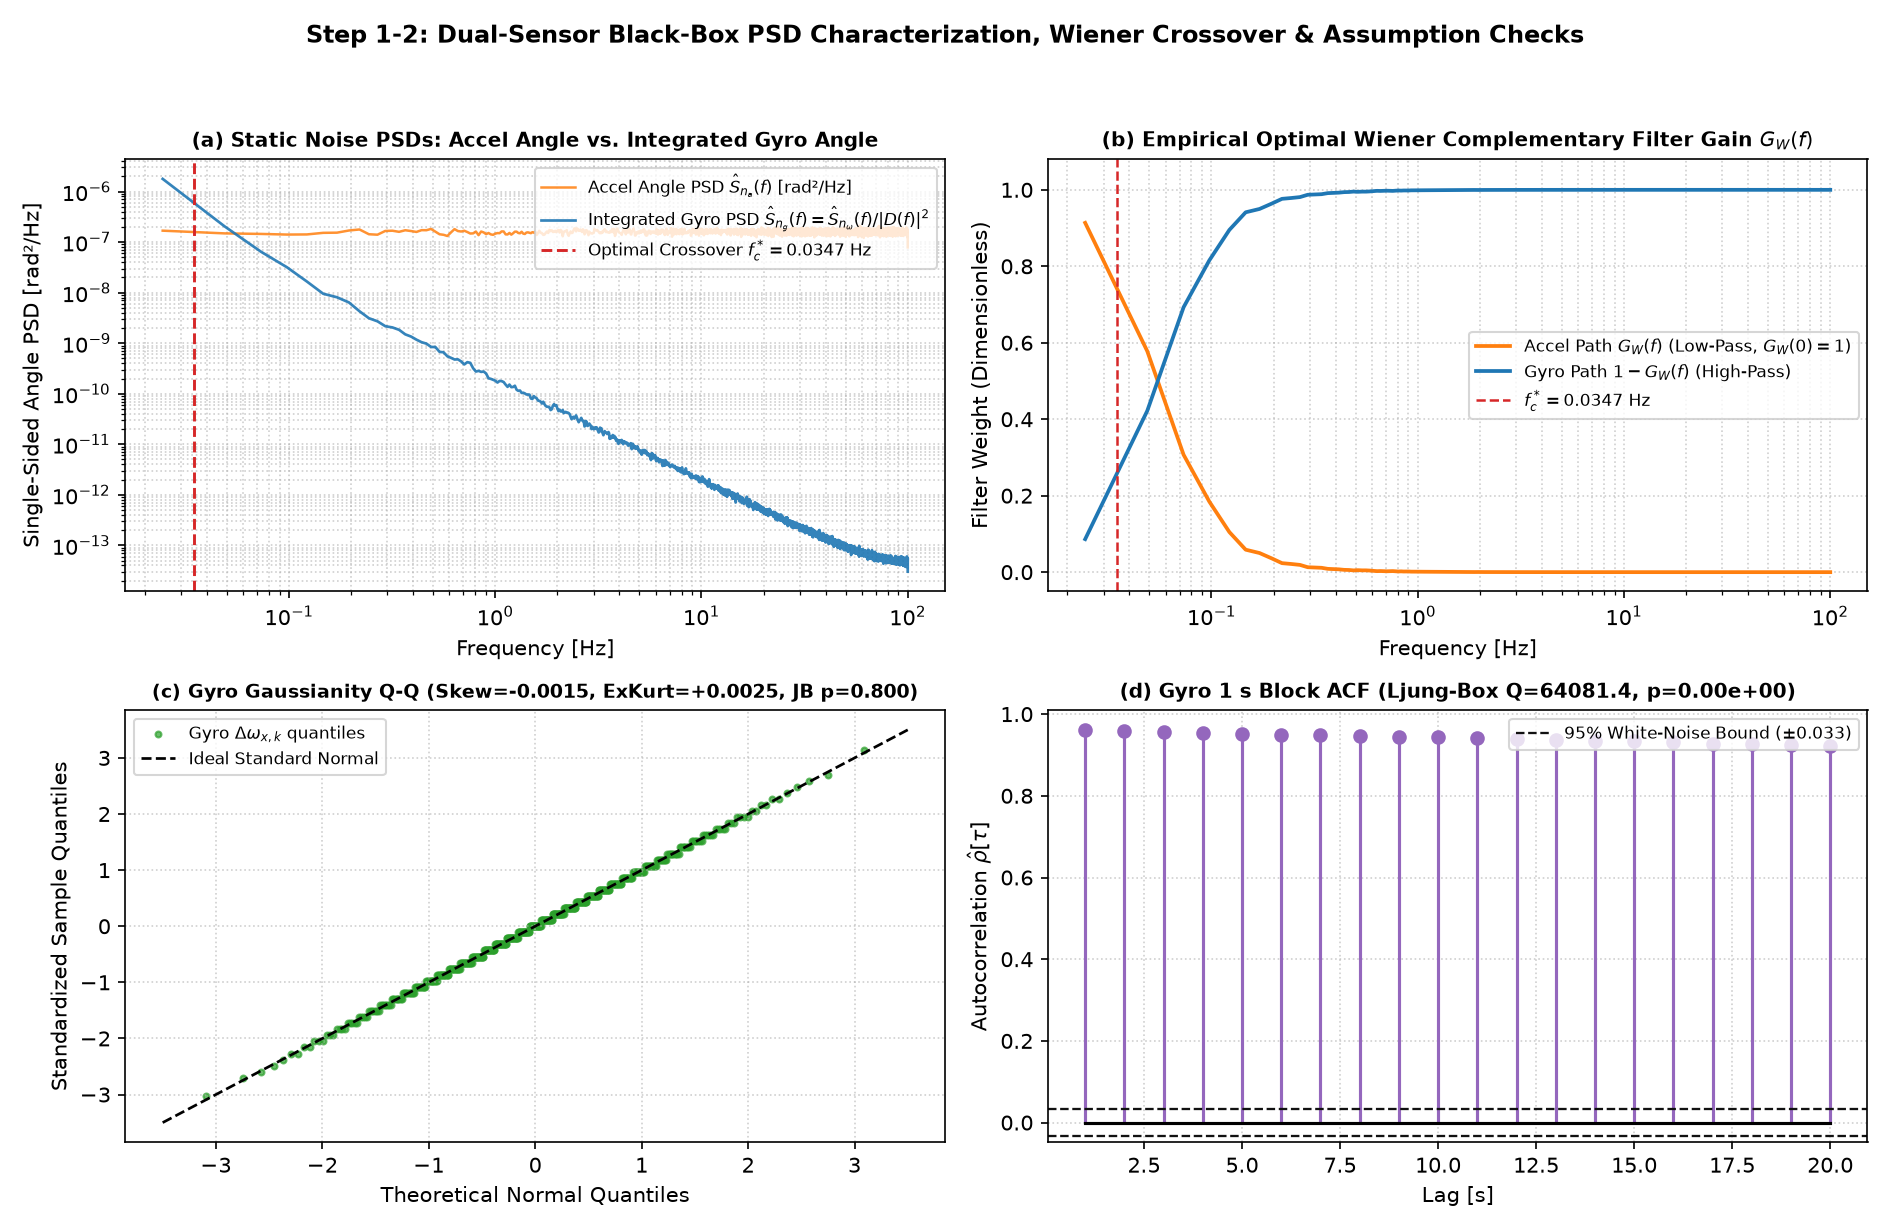
\includegraphics[width=\linewidth,height=6.7cm,keepaspectratio]{assets/fig1_dual_assumptions_and_wiener_psd.png}
    \end{column}
    \begin{column}{0.38\textwidth}
      {\fontsize{6.9}{8.5}\selectfont
      \begin{tabular}{p{1.45cm} p{2.20cm} p{1.35cm}}
        \rowcolor{hustred}
        \textbf{\color{white}Giả thiết} & \textbf{\color{white}Accel / Gyro} & \textbf{\color{white}Kết luận} \\
        1. Bão hòa & $\max|y|\ll 95\%$ FSR & \textbf{\color{greenaccent}Đạt} \\
        \rowcolor{lightbg}
        2. Kỳ vọng 0 & $t=-80.5 / +153.5$\newline (SE khối, $p\approx 0$) & \textbf{\color{hustred}Bác bỏ}\newline $\to$ Bù bias \\
        3. Chuẩn & JB trên $\Delta y_k$:\newline $p=0.576 / 0.800$ & \textbf{\color{greenaccent}Đạt chặt} \\
        \rowcolor{lightbg}
        4. Dừng WSS & 10 khối / 1 giờ:\newline TB trôi rõ rệt & \textbf{\color{amberaccent}Không dừng} \\
        5. Trắng? & Ljung--Box 1 s:\newline $Q=21552 / 64081$ & \textbf{\color{hustred}Nhiễu màu} \\
        \bottomrule
      \end{tabular}}
      \vspace{0.18cm}
      \hustcard[redtint]{hustred}{\linewidth}{Hàm ý trực tiếp cho thiết kế lọc}{%
        \begin{itemize}\setlength{\itemsep}{1.5pt}
          \item Hình (a): giao điểm PSD xác định tần số cắt tối ưu Wiener $f_c^* = 0.0347\text{ Hz}$.
          \item Hình (d): ACF $\approx 0.95$ khẳng định bắt buộc có trạng thái bias $b_k$ trong Kalman.
        \end{itemize}
      }
    \end{column}
  \end{columns}
\end{frame}

% ==============================================================================
% MAIN SLIDE 6 / 14: DUAL ALLAN DEVIATION & PARAMETER IDENTIFICATION
% ==============================================================================
\begin{frame}{2. Nhận dạng Tham số Nhiễu Hộp đen có Sai số (Accel \& Gyro)}
  \begin{center}
    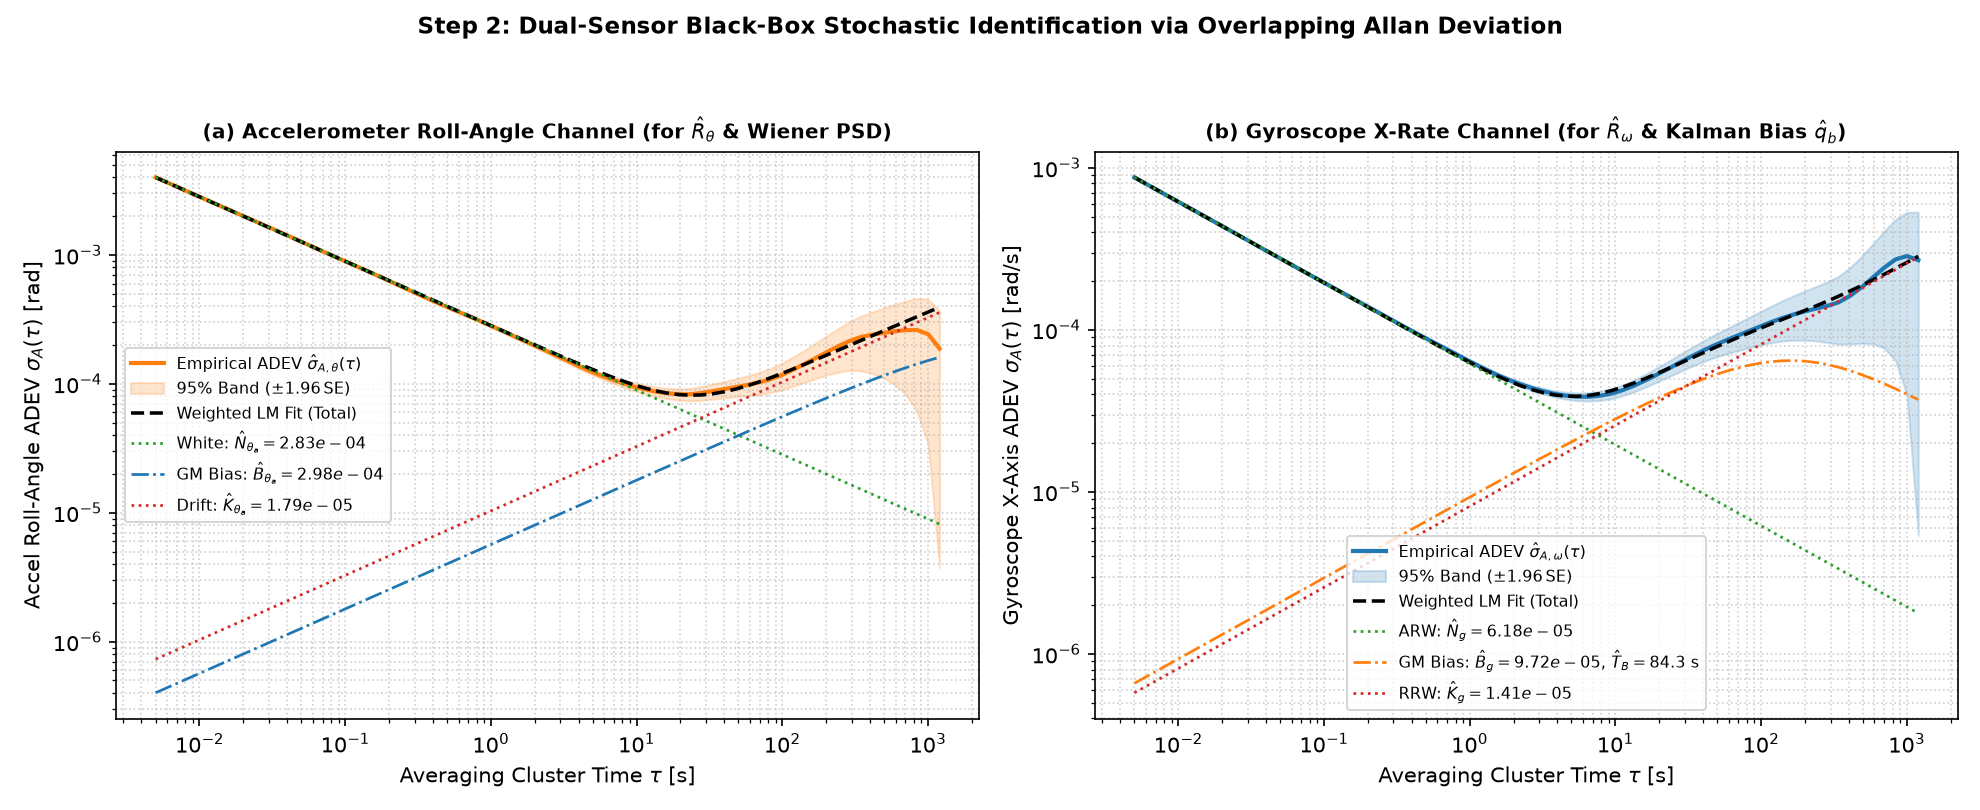
\includegraphics[width=0.92\textwidth,height=3.65cm,keepaspectratio]{assets/fig2_gyro_allan_identification.png}
  \end{center}
  \vspace{-0.15cm}
  {\fontsize{6.8}{8.3}\selectfont
  \begin{tabular}{p{2.7cm} p{4.25cm} p{2.25cm} p{1.45cm} p{3.15cm}}
    \rowcolor{hustred}
    \textbf{\color{white}Tham số nhận dạng} & \textbf{\color{white}Ước lượng hộp đen ($\pm$ SE / CI 95\%)} & \textbf{\color{white}Ẩn thật*} & \textbf{\color{white}Sai lệch} & \textbf{\color{white}Vai trò trong bộ lọc} \\
    \rowcolor{greentint}
    Accel $\hat{\sigma}_{\theta_a}$ / $\hat{R}_\theta$ & $0.2292^\circ$ $[0.2287, 0.2297]$ ($1.600\times 10^{-5}$) & $0.2292^\circ$ & \textbf{0.01\%} & $\mathbf{R}_{11}$ (Kalman) \& $\hat{S}_{n_a}$ \\
    Gyro $\hat{b}_{g,0}$ ($10\text{ s}$) & $0.01500 \pm 0.00010\text{ rad/s}$ (SE khối) & $0.01500\text{ rad/s}$ & \textbf{0.01\%} & Hiệu chuẩn / Khởi tạo $b_0$ \\
    \rowcolor{greentint}
    Gyro $\hat{\sigma}_\omega$ / $\hat{N}_g$ & $8.722\times 10^{-4}$ / $(6.175\pm 0.003)\times 10^{-5}$ & $8.727\times 10^{-4}$ & \textbf{0.05\%} & $\mathbf{R}_{22}$ (Kalman) \& $\omega_c^*$ \\
    Gyro $\hat{B}_g$ / $\hat{T}_{B,g}$ & $(9.72\pm 3.66)\times 10^{-5}$ / $84.3\pm 49.4\text{ s}$ & $1.20\times 10^{-4}$ / $100\text{ s}$ & \textbf{0.3--0.6 SE} & Khuếch tán $\hat{q}_{B,g}$ \\
    \rowcolor{lightbg}
    Gyro $\hat{K}_g$ (RRW) & $(1.41\pm 0.22)\times 10^{-5}\text{ rad/s}^{3/2}$ & $1.00\times 10^{-5}$ & \textbf{1.9 SE} & Khuếch tán $\hat{q}_{K,g}$ \\
    \bottomrule
  \end{tabular}}
  \vspace{0.06cm}
  {\fontsize{6.2}{7.4}\selectfont\color{mutedtext}*Giá trị ẩn thật trong \texttt{default.yaml} CHỈ dùng đối chiếu hậu kiểm — không nạp vào bộ lọc. Toàn bộ 8/8 tham số nhận dạng hộp đen đều chứa giá trị thật trong khoảng tin cậy 95\%.}
\end{frame}

% ==============================================================================
% MAIN SLIDE 7 / 14: METHOD 1 — OPTIMAL WIENER COMPLEMENTARY FILTER
% ==============================================================================
\begin{frame}{3. Phương án 1: Bộ lọc Bù Tối ưu kiểu Wiener (Miền tần số)}
  \begin{columns}[T,totalwidth=\textwidth]
    \begin{column}{0.49\textwidth}
      \hustcard[greentint]{greenaccent}{\linewidth}{A. Dẫn xuất Hàm truyền Tối ưu từ PSD Tĩnh}{%
        \begin{itemize}\setlength{\itemsep}{1.8pt}
          \item \textbf{Cấu trúc không méo tín hiệu $\theta(t)$:} Tổng hệ số 2 nhánh bằng 1 $\Rightarrow$ sai số $E(f)$ độc lập hoàn toàn với $\theta(t)$!
          \item \textbf{Cực tiểu hóa MMSE:} $\min_G \big(|G|^2 S_{n_a} + |1-G|^2 S_{n_g}\big)$ với $S_{n_g}(f) = S_{n_\omega}(f)/|D(f)|^2$:
        \end{itemize}
        \vspace{-0.12cm}
        \begin{align*}
          \hat{\Theta}(f) &= G(f)\,Z_a(f) + (1 - G(f))\,Z_g(f) \\
          E(f) &= G(f)\,N_a(f) + (1 - G(f))\,N_g(f) \\
          G_W(f) &= \frac{S_{n_\omega}(f)}{S_{n_\omega}(f) + |D(f)|^2\,S_{n_a}(f)},\;\; D(f)=\frac{1-e^{-j2\pi f\Delta t}}{\Delta t}
        \end{align*}
      }
    \end{column}
    \begin{column}{0.49\textwidth}
      \hustcard[lightbg]{hustred}{\linewidth}{B. Dạng Không tích phân dốc \& Bản Nhân quả}{%
        \begin{itemize}\setlength{\itemsep}{1pt}
          \item \textbf{Triệt bias DC không tạo đường dốc:} $H_{\text{gyr}}(0)=0$ chặn tuyệt đối bias hằng số của gyro mà không tích phân gây nhảy biên FFT (đệm biên đối xứng chẵn/lẻ).
          \item \textbf{Bản nhân quả bậc 1:} Phân tích phổ cho $\omega_c^* = 0.218\text{ rad/s}$ ($\alpha^*=0.99891$), nhưng chịu lệch tĩnh $\Delta\theta_{\text{ss}} = b_g/\omega_c^*$!
        \end{itemize}
        \vspace{-0.18cm}
        {\fontsize{6.9}{8.2}\selectfont
        \begin{align*}
          \hat{\Theta}(f) &= G_W(f)\,Z_a(f) + H_{\text{gyr}}(f)\,\tilde{\Omega}_x(f) \\
          H_{\text{gyr}}(f) &= \frac{D^*(f)\,S_{n_a}(f)}{S_{n_\omega}(f) + |D(f)|^2 S_{n_a}(f)} \;\Longrightarrow\; H_{\text{gyr}}(0) = 0 \\
          \omega_c^* &= \sqrt{\frac{S_\omega}{S_{\theta_a}}} = \frac{\hat{N}_g}{\hat{N}_{\theta_a}} = 0.218\text{ rad/s}\;(f_c^* = 0.0347\text{ Hz})
        \end{align*}}
        \vspace{-0.22cm}
      }
    \end{column}
  \end{columns}

  \vspace{0.10cm}
  \takeaway[greentint]{greenaccent}{Dự báo lý thuyết từ PSD tĩnh (không cần ground truth): $\mathrm{RMSE}_{\text{theo}} = \sqrt{\int_0^{f_s/2} G_W(f)S_{n_a}(f)\,df} = 0.0056^\circ$ — không cần chỉnh tay hệ số $\alpha$ như Baseline.}
\end{frame}

% ==============================================================================
% MAIN SLIDE 8 / 14: METHOD 2 — 4-STATE KALMAN FILTER [u, u', u'', b]^T
% ==============================================================================
\begin{frame}{3. Phương án 2: Bộ lọc Kalman 4 Trạng thái $\mathbf{x}_k = [u_k, \dot{u}_k, \ddot{u}_k, b_k]^T$}
  \begin{columns}[T,totalwidth=\textwidth]
    \begin{column}{0.56\textwidth}
      \hustcard[bluetint]{blueaccent}{\linewidth}{Mô hình Không gian Trạng thái CA + Bias (Hợp nhất Đo 2D)}{%
        \textbf{4 biến trạng thái:} $u_k=\theta_k$ (góc Roll), $\dot{u}_k=\dot{\theta}_k$ (vận tốc góc), $\ddot{u}_k=\ddot{\theta}_k$ (gia tốc góc), $b_k = b_0+x_{B,k}+x_{K,k}$ (tổng bias gyro).
        \vspace{-0.20cm}
        {\renewcommand{\arraystretch}{0.95}\fontsize{6.9}{8.2}\selectfont
        \begin{align*}
          \mathbf{x}_k &= \begin{bmatrix}1 & \Delta t & \tfrac{1}{2}\Delta t^2 & 0 \\ 0 & 1 & \Delta t & 0 \\ 0 & 0 & 1 & 0 \\ 0 & 0 & 0 & 1\end{bmatrix}\mathbf{x}_{k-1} + \mathbf{w}_k \\
          \mathbf{y}_k &= \begin{bmatrix}\theta_{\text{acc,cal}}[k] \\ \tilde{\omega}_{x,k}\end{bmatrix} = \begin{bmatrix}1 & 0 & 0 & 0 \\ 0 & 1 & 0 & 1\end{bmatrix}\mathbf{x}_k + \mathbf{v}_k \\
          \mathbf{Q} &= \mathrm{blkdiag}\!\big(q_u\mathbf{Q}_{\text{CA}},\,\hat{q}_{B,g}+\hat{q}_{K,g}\big), \quad \mathbf{R} = \mathrm{diag}(\hat{R}_\theta, \hat{R}_\omega)
        \end{align*}}
        \vspace{-0.24cm}
      }
    \end{column}
    \begin{column}{0.42\textwidth}
      \hustcard[lightbg]{blueaccent}{\linewidth}{1. Quan sát được Toàn hạng ($\mathrm{rank}=4$)}{%
        {\fontsize{6.9}{8.5}\selectfont Hàng 1 đo $u_k \to$ xác định $\dot{u}_k,\ddot{u}_k$; hàng 2 đo $\dot{u}_k + b_k \to$ tách hoàn toàn bias $b_k$. Đặt $F_{44}=1$ tránh kéo co (\textit{shrinkage}) bias nhiệt về 0.}
      }
      \vspace{0.09cm}
      \hustcard[redtint]{hustred}{\linewidth}{2. Tinh chỉnh $q_u$ bằng Gyro-MLE (0 GT)}{%
        {\fontsize{6.9}{8.5}\selectfont Cực đại hóa log-likelihood phần dư kênh gyro $(\nu_g, S_{gg})$ $\Rightarrow$ khớp đúng động học xoay \& \textbf{miễn nhiễm rung ngang} trên gia tốc kế!}
      }
      \vspace{0.09cm}
      \hustcard[greentint]{greenaccent}{\linewidth}{3. Ổn định số \& Thời gian thực}{%
        {\fontsize{6.9}{8.5}\selectfont Cập nhật hiệp phương sai dạng Joseph đối xứng dương; tốc độ \textbf{0.0146 ms/mẫu} ($>340\times$ nhanh hơn chu kỳ $5\text{ ms}$).}
      }
    \end{column}
  \end{columns}

  \vspace{0.10cm}
  \takeaway[bluetint]{blueaccent}{Toàn bộ $(\hat{R}_\theta, \hat{R}_\omega, \hat{q}_{B,g}, \hat{q}_{K,g})$ nạp trực tiếp từ nhận dạng hộp đen Bước 2 — lọc mượt đồng thời góc $u_k$, tốc độ góc $\dot{u}_k$, gia tốc góc $\ddot{u}_k$ \& bias $b_k$ trực tuyến từ $t=0$.}
\end{frame}

% ==============================================================================
% MAIN SLIDE 9 / 14: 4 TEST SCENARIOS & EVALUATION FRAMEWORK
% ==============================================================================
\begin{frame}{4. Thiết kế 4 Kịch bản Thực nghiệm \& Khung Đánh giá}
  \begin{columns}[T,totalwidth=\textwidth]
    \begin{column}{0.24\textwidth}
      \hustcard[bluetint]{blueaccent}{\linewidth}{S1: Static (30 s)}{%
        \textbf{Đầu vào:} $\theta(t)=0^\circ$, $a_{\text{lin}}=0$.\\[3pt]
        \textbf{Mục tiêu:} Kiểm chứng độ phẳng tĩnh, mức giảm nhiễu \& tính nhất quán NIS/2 chuẩn.
      }
    \end{column}
    \begin{column}{0.24\textwidth}
      \hustcard[greentint]{greenaccent}{\linewidth}{S2: Sin $12^\circ$ (20 s)}{%
        \textbf{Đầu vào:} $12^\circ\sin(2\pi\cdot 0.3t)$.\\[3pt]
        \textbf{Mục tiêu:} Kiểm chứng vùng tuyến tính hóa góc nhỏ \& phát hiện sai số hệ số tỉ lệ ẩn.
      }
    \end{column}
    \begin{column}{0.24\textwidth}
      \hustcard[redtint]{hustred}{\linewidth}{S3: Rung 4 Hz (20 s)}{%
        \textbf{Đầu vào:} $10^\circ@0.25\text{Hz}+4^\circ@1.2\text{Hz}$ + rung $1.5\sin(2\pi\cdot 4t)$.\\[3pt]
        \textbf{Mục tiêu:} Góc giả $\sim 8.7^\circ$ kiểm chứng triệt rung ngang.
      }
    \end{column}
    \begin{column}{0.24\textwidth}
      \hustcard[ambertint]{amberaccent}{\linewidth}{S4: Drift 180 s}{%
        \textbf{Đầu vào:} $10^\circ@0.15\text{Hz}$ + bước nhảy bias $+0.008\text{ rad/s}$.\\[3pt]
        \textbf{Mục tiêu:} Kiểm chứng khử trôi dài hạn \& hội tụ bias online.
      }
    \end{column}
  \end{columns}

  \vspace{0.25cm}
  \begin{columns}[T,totalwidth=\textwidth]
    \begin{column}{0.49\textwidth}
      \hustcard[lightbg]{blueaccent}{\linewidth}{Trục đánh giá 1: KHÔNG cần Ground Truth (Vận hành thực tế)}{%
        \begin{itemize}\setlength{\itemsep}{2.5pt}
          \item \textbf{Normalized Innovation Squared ($\overline{\text{NIS}}/2$):} Kiểm tra trung bình $\frac{1}{2}\boldsymbol{\nu}_k^T\mathbf{S}_k^{-1}\boldsymbol{\nu}_k$ nằm trong dải 95\% phân bố $\chi^2$ quanh $1.0$.
          \item \textbf{Tính trắng của phần dư:} Kiểm định Ljung--Box ($L=20$) trên ACF phần dư góc.
          \item \textbf{Bất định hậu nghiệm:} Theo dõi độ lệch chuẩn $\sqrt{P_{uu}}$ và $\sqrt{P_{bb}}$ hội tụ.
        \end{itemize}
      }
    \end{column}
    \begin{column}{0.49\textwidth}
      \hustcard[lightbg]{hustred}{\linewidth}{Trục đánh giá 2: CÓ Ground Truth (Chấm điểm định lượng)}{%
        \begin{itemize}\setlength{\itemsep}{2.5pt}
          \item \textbf{Benchmark Monte Carlo độc lập:} Chạy lặp $20\text{ seed}$ (S1--S3) \& $10\text{ seed}$ (S4) báo cáo $\text{RMSE} = \text{Mean} \pm 1\text{ SD}$.
          \item \textbf{Chỉ số bổ trợ:} MAE, sai số trung bình (Bias), độ trễ pha (Lag ms), thời gian chạy/mẫu.
          \item \textbf{2 Stress-Tests độ bền vững:} Quét biên độ rung ngang $0\to 3.0\text{ m/s}^2$ \& bước nhảy bias nhiệt $0\to 2.0^\circ/\text{s}$.
        \end{itemize}
      }
    \end{column}
  \end{columns}
\end{frame}

% ==============================================================================
% MAIN SLIDE 10 / 14: SCENARIO 3 RESULTS — VIBRATION REJECTION
% ==============================================================================
\begin{frame}{4. Kết quả S3: Triệt Rung động Ngang — Wiener \& Kalman Áp đảo}
  \begin{columns}[T,totalwidth=\textwidth]
    \begin{column}{0.68\textwidth}
      \centering
      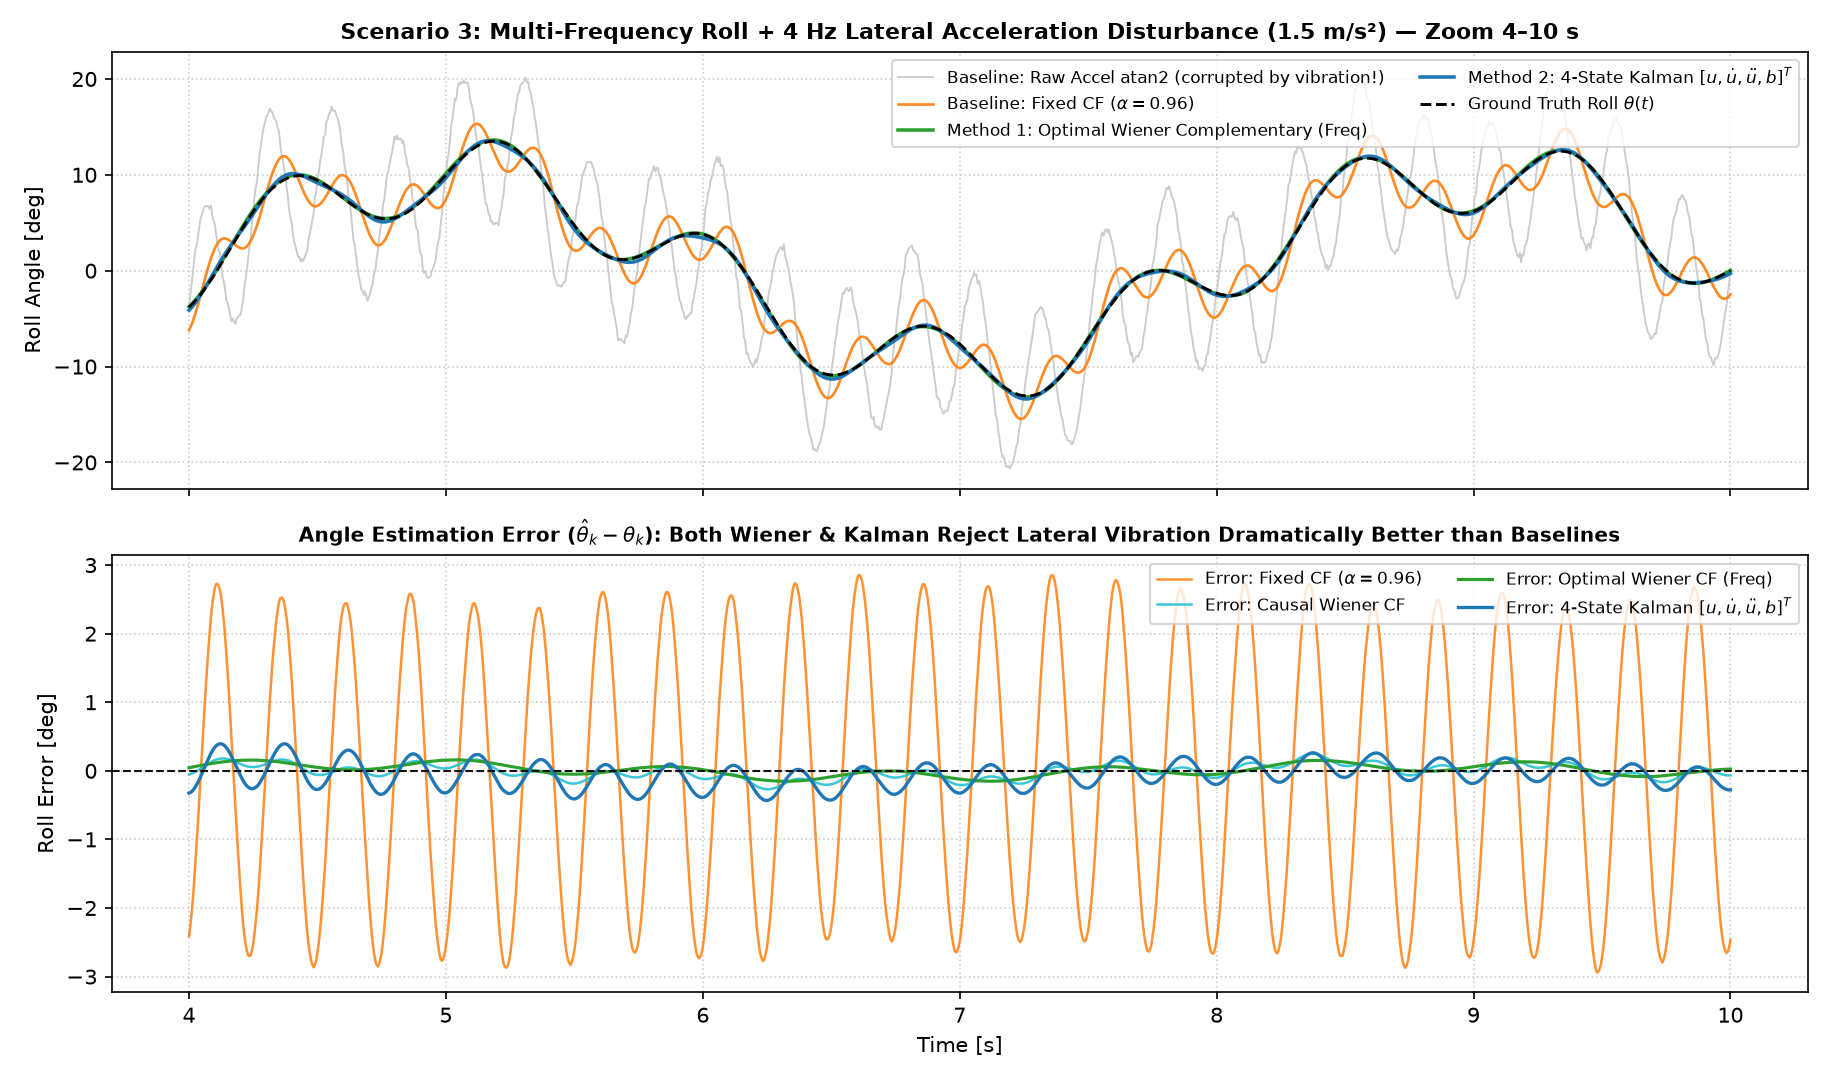
\includegraphics[width=\linewidth,height=6.75cm,keepaspectratio]{assets/fig3_vibration_comparison_s3.png}
    \end{column}
    \begin{column}{0.30\textwidth}
      \kpicard{mutedtext}{lightbg}{Baseline: Raw Accel ($\mathrm{atan2}$)}{$6.089^\circ \pm 0.004^\circ$}{Vỡ trận do rung 4 Hz (góc giả $\pm 10^\circ$)}\\[4pt]
      \kpicard{amberaccent}{ambertint}{Baseline: Fixed CF ($\alpha=0.96$)}{$1.886^\circ \pm 0.001^\circ$}{Lọt rung $\pm 2.8^\circ$ do $f_c=1.33\text{ Hz}$ quá cao}\\[4pt]
      \kpicard{greenaccent}{greentint}{PA 1: Optimal Wiener (Freq)}{$0.088^\circ \pm 0.002^\circ$}{Giảm \textbf{69$\times$} so với Accel | Hơn CF \textbf{21$\times$}}\\[4pt]
      \kpicard{blueaccent}{bluetint}{PA 2: Kalman 4 Trạng thái}{$0.284^\circ \pm 0.003^\circ$}{Giảm \textbf{21.4$\times$} | $\text{NIS}/2=353$ cảnh báo rung!}
    \end{column}
  \end{columns}
\end{frame}

% ==============================================================================
% MAIN SLIDE 11 / 14: SCENARIO 4 RESULTS — LONG-TERM DRIFT & BIAS TRACKING
% ==============================================================================
\begin{frame}{4. Kết quả S4: Khử Trôi Dài hạn (180 s) \& Hội tụ Bias Online}
  \begin{columns}[T,totalwidth=\textwidth]
    \begin{column}{0.68\textwidth}
      \centering
      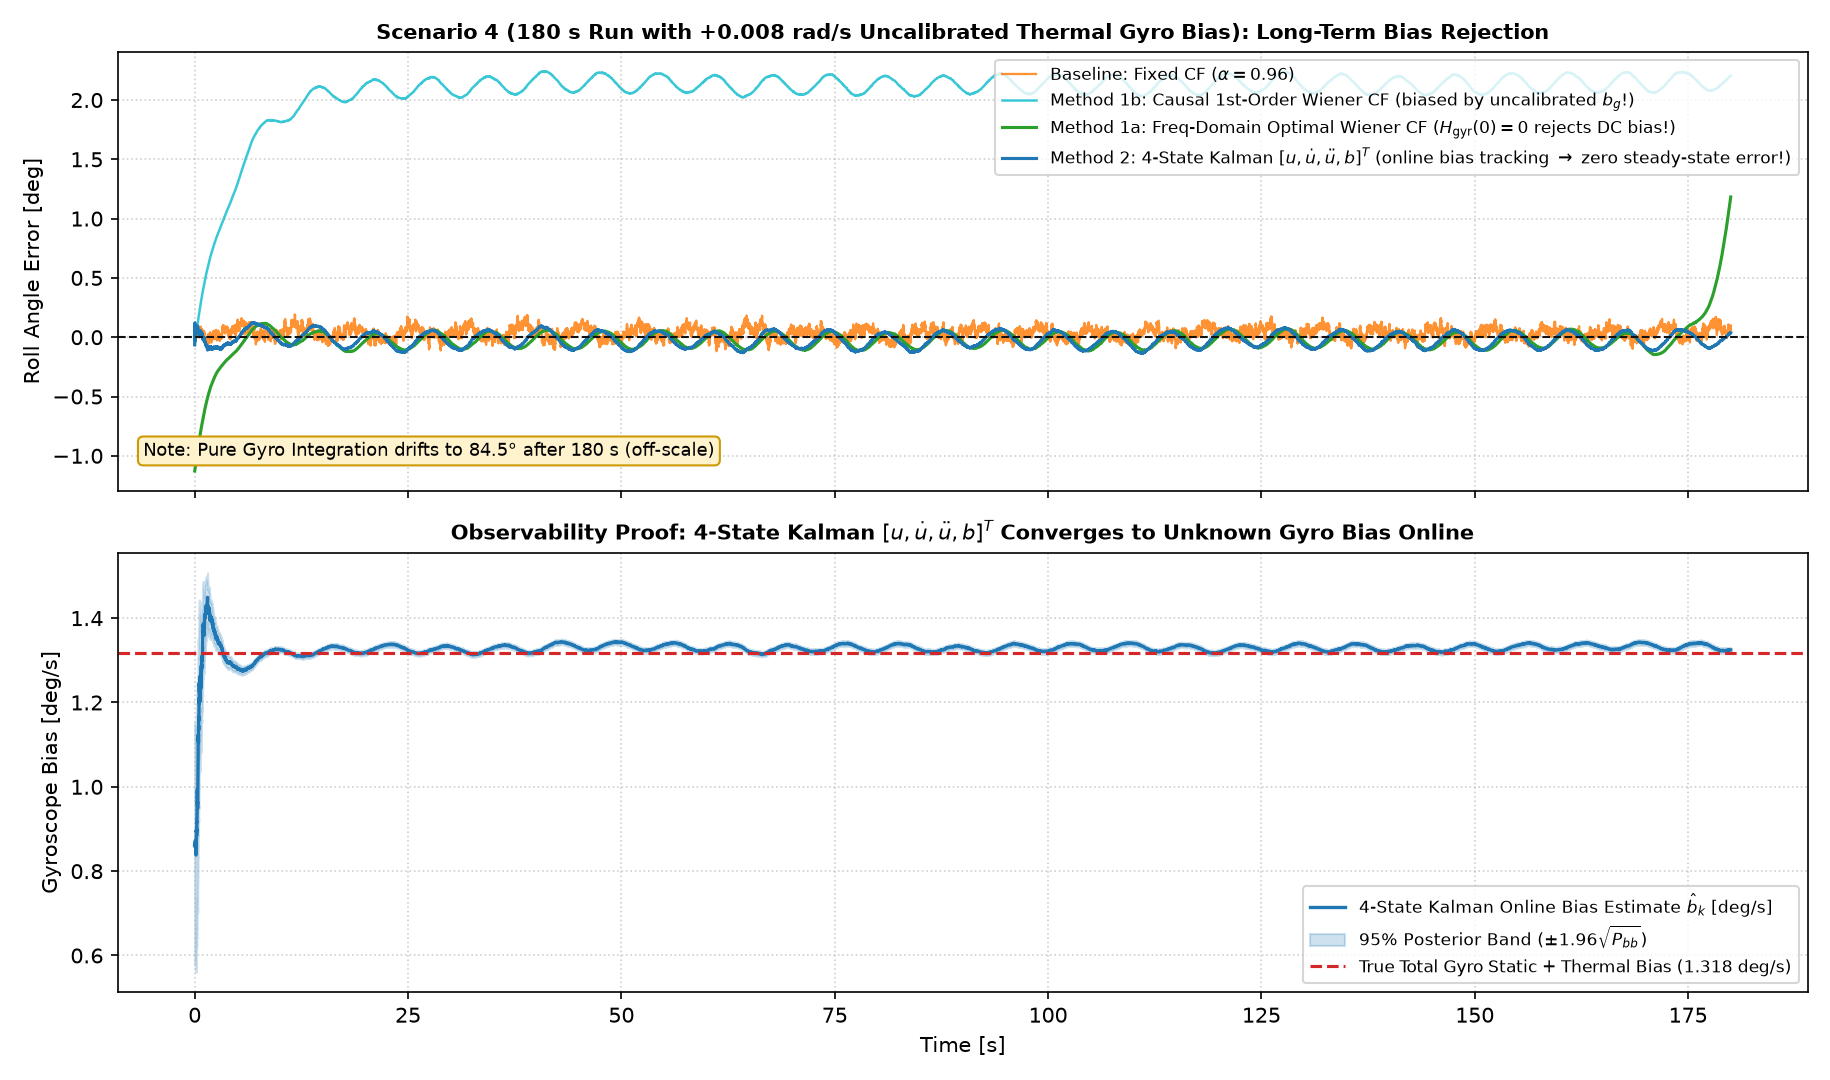
\includegraphics[width=\linewidth,height=6.75cm,keepaspectratio]{assets/fig4_drift_and_bias_tracking_s4.png}
    \end{column}
    \begin{column}{0.30\textwidth}
      \kpicard{hustred}{redtint}{Baseline: Raw Gyro Integration}{$48.39^\circ$ {\scriptsize(cuối $84.5^\circ$)}}{Trôi góc tuyến tính không kiểm soát}\\[2pt]
      \kpicard{amberaccent}{ambertint}{PA 1b: Wiener Nhân quả bậc 1}{$2.080^\circ \pm 0.028^\circ$}{Lệch tĩnh khớp lý thuyết $b_g/\omega_c^*\approx 2.10^\circ$}\\[2pt]
      \kpicard{greenaccent}{greentint}{PA 1a: Wiener Miền tần số}{$0.101^\circ \pm 0.002^\circ$}{$H_{\text{gyr}}(0)=0$ chặn DC (chỉ còn hiệu ứng biên)}\\[2pt]
      \kpicard{blueaccent}{bluetint}{PA 2: Kalman 4 Trạng thái}{$0.062^\circ \pm 0.002^\circ$}{\textbf{Tốt nhất!} Khóa $\hat{b}_k=0.02312$ vs $0.02300$}
    \end{column}
  \end{columns}
\end{frame}

% ==============================================================================
% MAIN SLIDE 12 / 14: NO-GROUND-TRUTH DIAGNOSTICS (NIS & INNOVATION)
% ==============================================================================
\begin{frame}{4. Chẩn đoán Không cần Ground Truth: Phát hiện Lỗi Ẩn qua NIS/2}
  \begin{columns}[T,totalwidth=\textwidth]
    \begin{column}{0.60\textwidth}
      \centering
      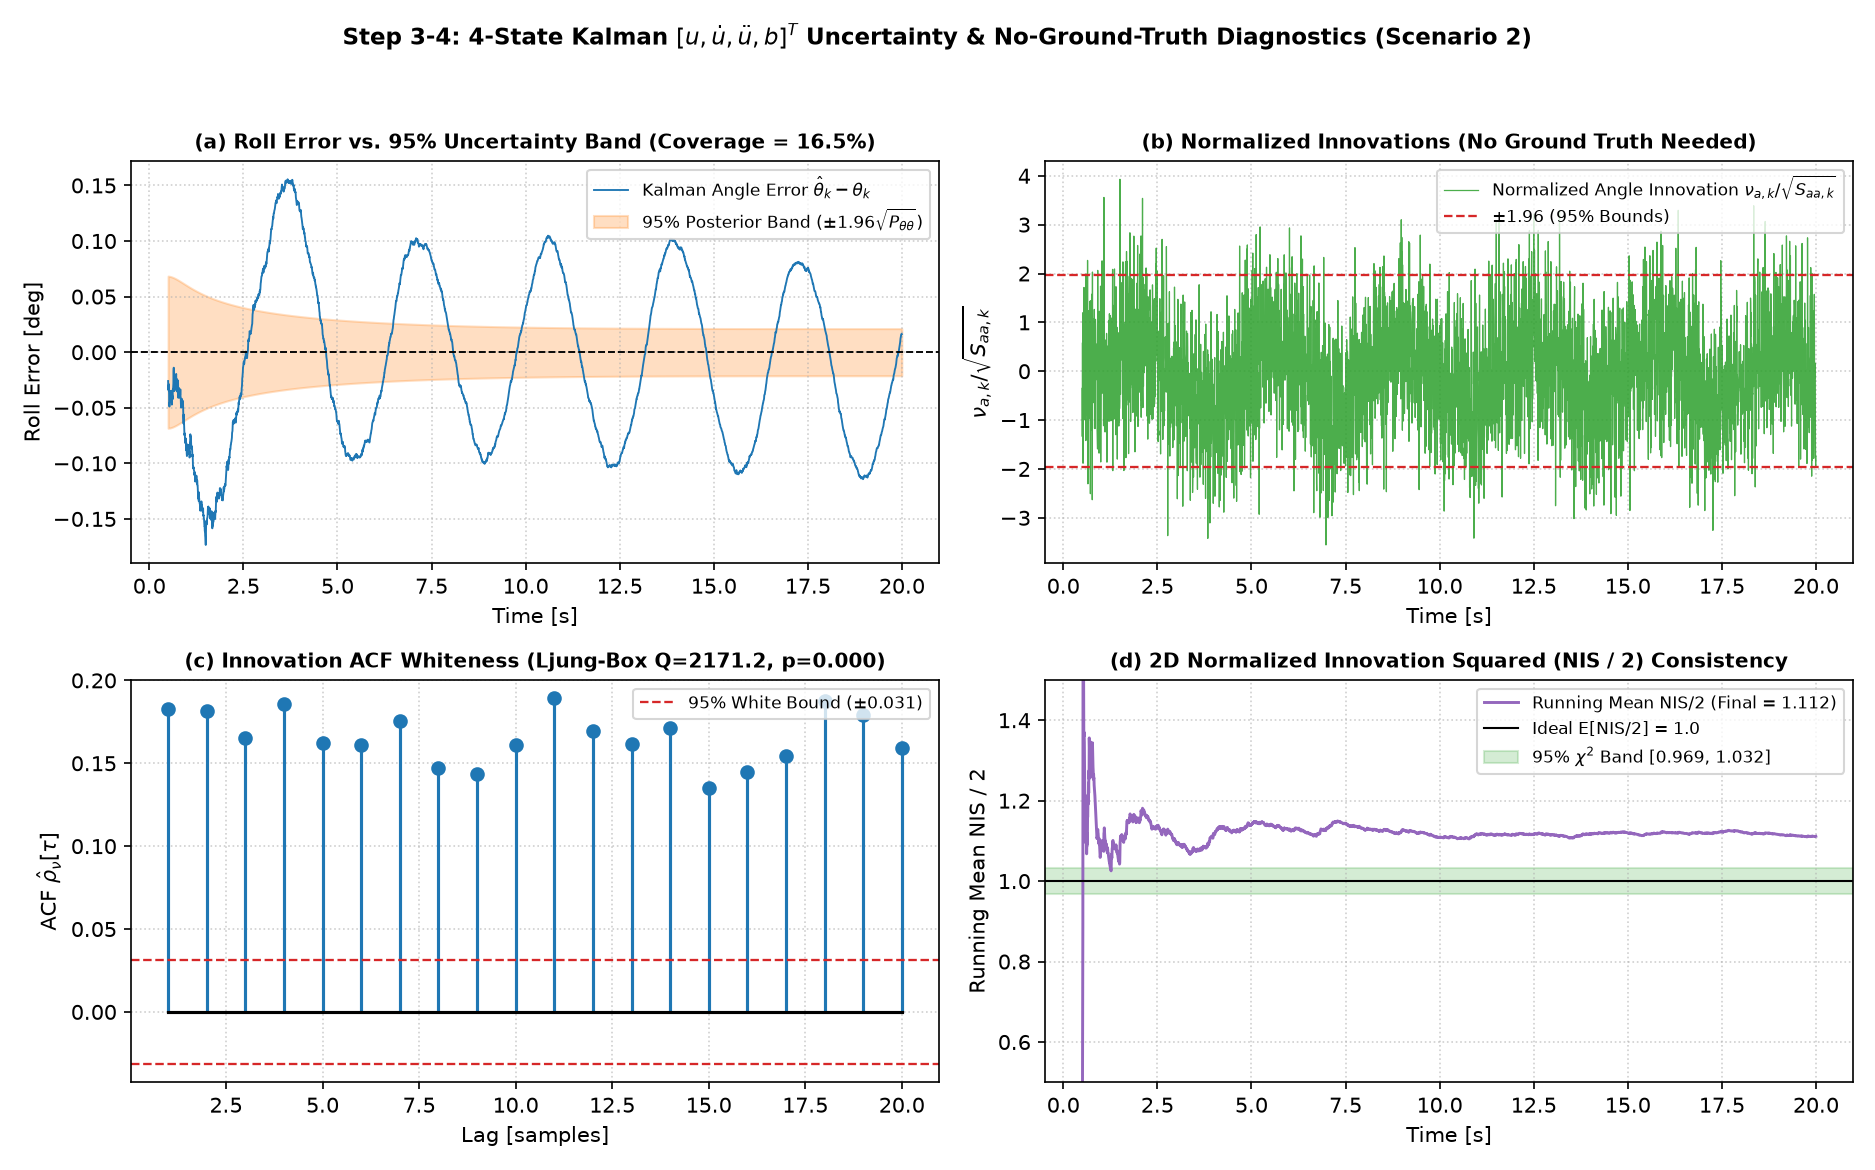
\includegraphics[width=\linewidth,height=6.75cm,keepaspectratio]{assets/fig5_kalman_consistency_s2.png}
    \end{column}
    \begin{column}{0.39\textwidth}
      {\fontsize{6.9}{8.5}\selectfont
      \begin{tabular}{p{1.40cm} p{1.00cm} p{0.72cm} p{2.05cm}}
        \rowcolor{hustred}
        \textbf{\color{white}Kịch bản} & \textbf{\color{white}NIS/2} & \textbf{\color{white}LB $p$} & \textbf{\color{white}Chẩn đoán} \\
        \rowcolor{greentint}
        S1: Tĩnh & \textbf{1.002} & 0.100 & Nhất quán chuẩn \\
        \rowcolor{ambertint}
        S2: Sin $12^\circ$ & \textbf{1.112} & 0.000 & Lộ sai số tỉ lệ ẩn \\
        \rowcolor{redtint}
        S3: Rung & \textbf{353.4} & 0.000 & Cảnh báo rung ngang \\
        S4: 180 s & 1.064 & 0.000 & Khóa bias 0.5\% err \\
        \bottomrule
      \end{tabular}}
      \vspace{0.20cm}
      \hustcard[redtint]{hustred}{\linewidth}{Phát hiện kỹ thuật sâu sắc trên S2}{%
        \begin{itemize}\setlength{\itemsep}{2pt}
          \item \textbf{S1 ($\omega=0$):} Sai số hệ số tỉ lệ gyro không kích hoạt $\Rightarrow \overline{\text{NIS}}/2 = 1.002$ nhất quán tuyệt đối.
          \item \textbf{S2 ($\pm 12^\circ$):} Sai số hệ số tỉ lệ ẩn ($+0.8\%$) sinh sóng sin $0.3\text{ Hz}$ biên độ $\sim 0.10^\circ$ vượt dải nhiễu ngẫu nhiên $\pm 0.025^\circ$.
          \item \textbf{Ý nghĩa:} Chính NIS/2 \& ACF tự phát hiện lỗi hiệu chuẩn động mà không cần ground truth!
        \end{itemize}
      }
    \end{column}
  \end{columns}
\end{frame}

% ==============================================================================
% MAIN SLIDE 13 / 14: MONTE CARLO BENCHMARK & STRESS TESTS
% ==============================================================================
\begin{frame}{4. Benchmark Monte Carlo \& Kiểm tra Độ bền vững (Stress Tests)}
  \begin{columns}[T,totalwidth=\textwidth]
    \begin{column}{0.64\textwidth}
      \centering
      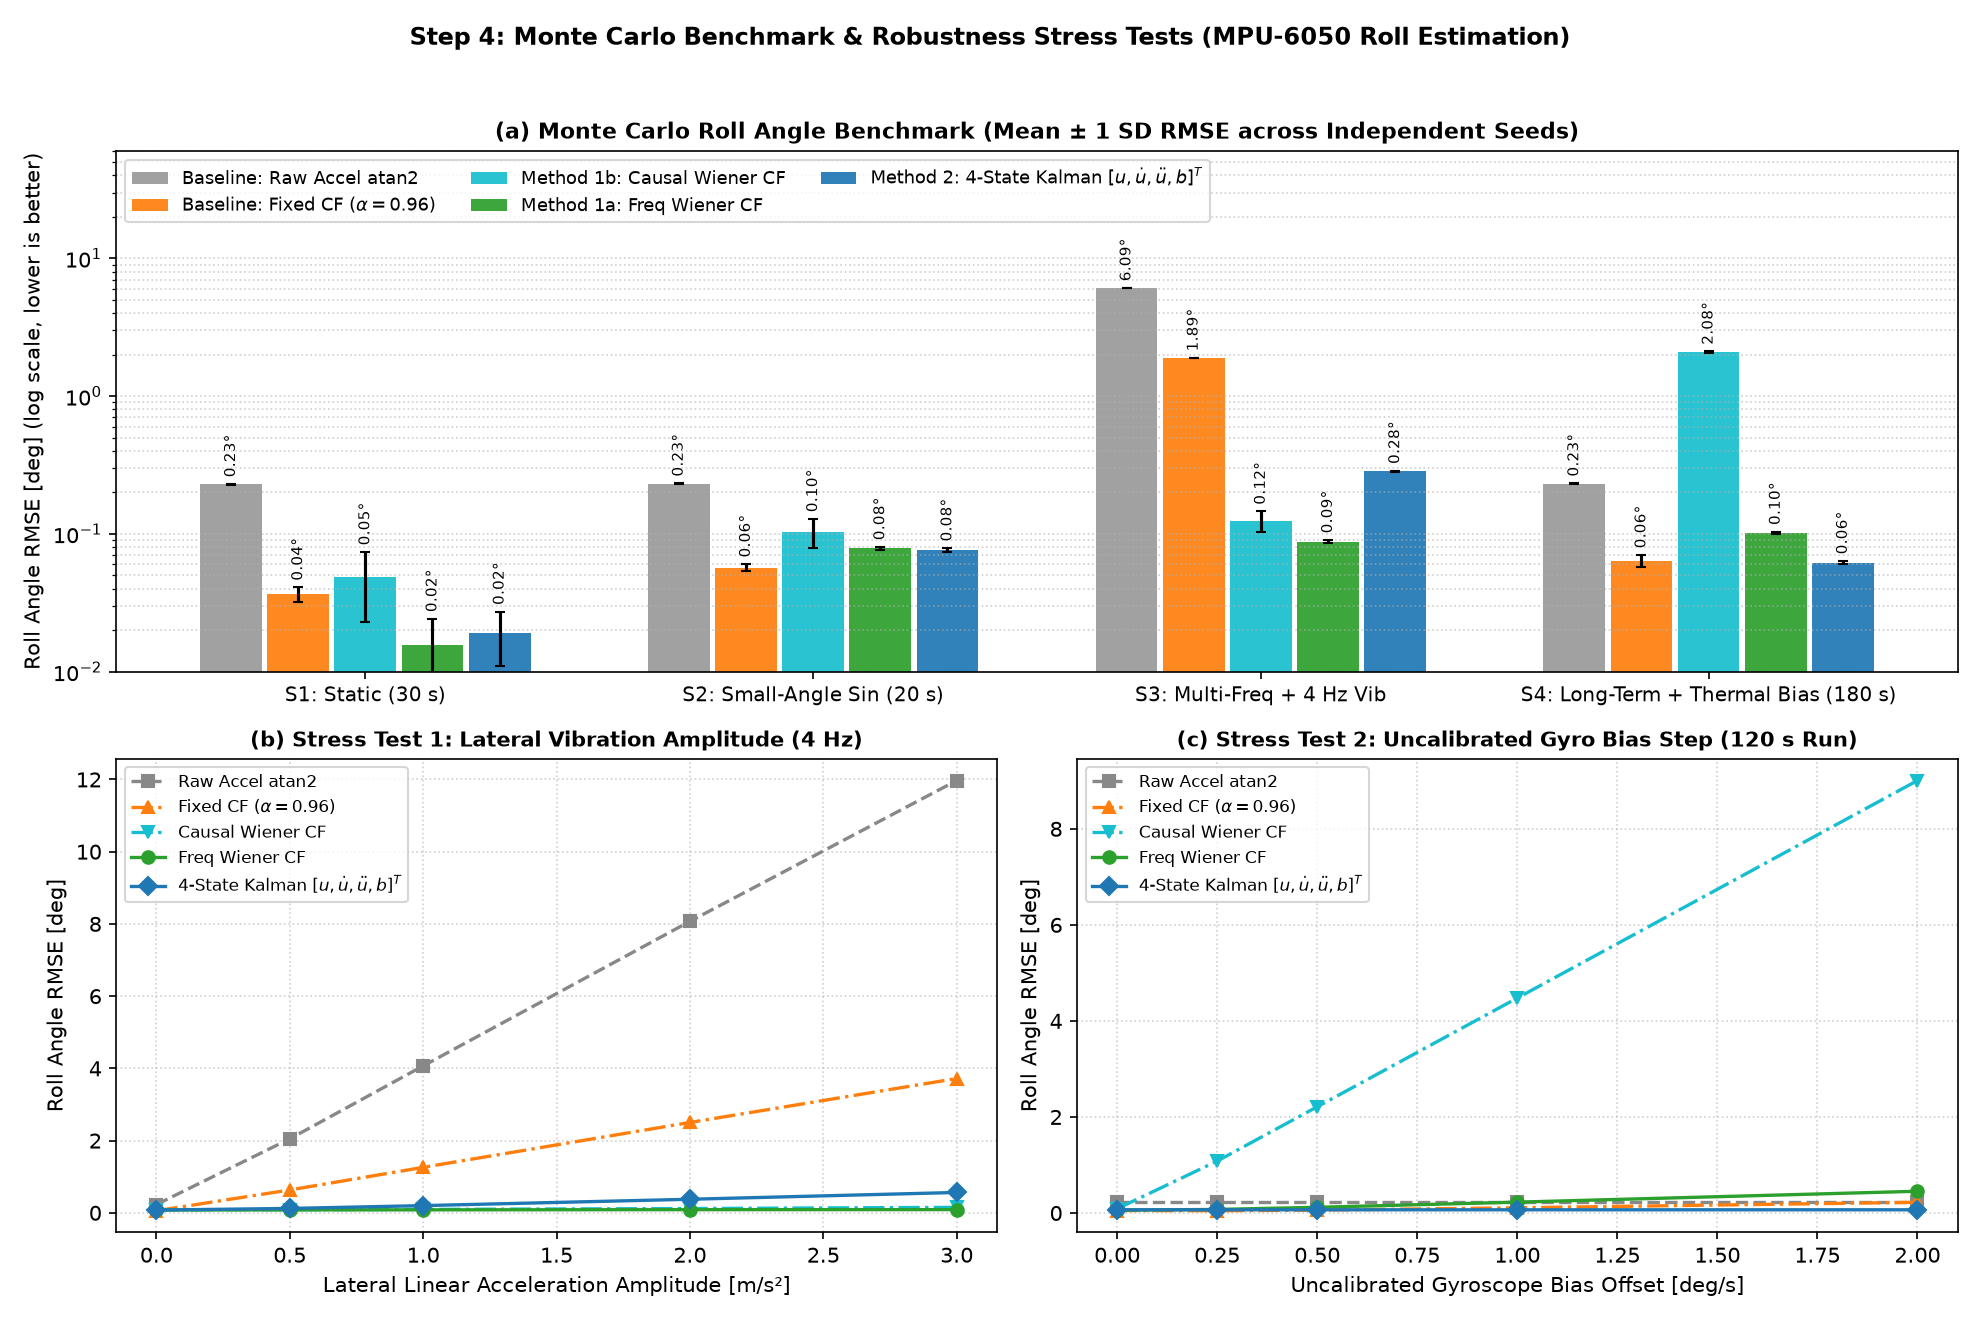
\includegraphics[width=\linewidth,height=6.75cm,keepaspectratio]{assets/fig6_montecarlo_and_stress.png}
    \end{column}
    \begin{column}{0.34\textwidth}
      \hustcard[greentint]{greenaccent}{\linewidth}{Stress Test 1: Rung $0 \to 3.0\text{ m/s}^2$}{%
        {\fontsize{6.7}{8.1}\selectfont
        \begin{itemize}\setlength{\itemsep}{1pt}
          \item Raw Accel vỡ lên $11.97^\circ$; Fixed CF lên $3.72^\circ$.
          \item \textbf{Wiener Freq:} $0.08^\circ \to 0.09^\circ$ (giảm \textbf{135$\times$}!).
          \item \textbf{Kalman 4-State:} $0.08^\circ \to 0.56^\circ$ (giảm \textbf{21$\times$}).
        \end{itemize}}
      }
      \vspace{0.08cm}
      \hustcard[bluetint]{blueaccent}{\linewidth}{Stress Test 2: Bias $0 \to 2.0^\circ/\text{s}$}{%
        {\fontsize{6.7}{8.1}\selectfont
        \begin{itemize}\setlength{\itemsep}{1pt}
          \item Wiener nhân quả tăng tuyến tính lên $9.01^\circ$.
          \item Wiener Freq tăng nhẹ $0.06^\circ \to 0.45^\circ$ (biên).
          \item \textbf{Kalman 4-State:} \textbf{BẤT BIẾN ở $0.067^\circ$!}
        \end{itemize}}
      }
      \vspace{0.08cm}
      \hustcard[ambertint]{amberaccent}{\linewidth}{Điểm sáng trên S2 \& S4}{%
        {\fontsize{6.7}{8.1}\selectfont Kalman 4 trạng thái đạt $0.076^\circ$ (S2) \& $0.062^\circ$ (S4) — vượt Wiener Freq nhờ lọc mượt đồng thời góc và tốc độ góc!}
      }
    \end{column}
  \end{columns}
\end{frame}

% ==============================================================================
% MAIN SLIDE 14 / 14: COMPARISON SUMMARY & FUTURE WORK
% ==============================================================================
\begin{frame}{5. So sánh Tổng kết Wiener vs. Kalman \& Hướng Mở rộng}
  \noindent{\fontsize{7.0}{8.6}\selectfont
  \begin{tabular}{p{3.0cm} p{5.6cm} p{5.6cm}}
    \rowcolor{hustred}
    \textbf{\color{white}Tiêu chí so sánh} & \textbf{\color{white}PA 1: Optimal Wiener CF (Miền tần số)} & \textbf{\color{white}PA 2: Kalman 4 Trạng thái $[u, \dot{u}, \ddot{u}, b]^T$} \\
    Chế độ vận hành & Xử lý theo khối (Offline, không nhân quả, zero-phase) & Đệ quy từng mẫu thời gian thực ($0.015\text{ ms/mẫu}\ll 5\text{ ms}$) \\
    \rowcolor{lightbg}
    Triệt rung động ngang & \textbf{Xuất sắc nhất} ($0.088^\circ$ ở $3\text{ m/s}^2$ — hơn Accel $135\times$) & Rất tốt ($0.28^\circ\text{--}0.56^\circ$, dễ nâng cấp Adaptive $R$ qua NIS) \\
    Chống bias nhiệt & Tốt ở phần thân ($H_{\text{gyr}}(0)=0$), có hiệu ứng biên nhẹ & \textbf{Xuất sắc tuyệt đối} ($0.067^\circ$ bất biến tới $2.0^\circ/\text{s}$) \\
    \rowcolor{lightbg}
    Bất định \& Tự chẩn đoán & Chỉ có $\mathrm{RMSE}_{\text{theo}}$ tĩnh & Dải $\pm 1.96\sqrt{P}$, ước lượng $\dot{u},\ddot{u},\hat{b}_k$ \& cảnh báo NIS/2 \\
    \rowcolor{bluetint}
    \textbf{Khuyến nghị ứng dụng} & \textbf{Hậu xử lý dữ liệu thí nghiệm / đo ghi sẵn (Offline)} & \textbf{Điều khiển vòng kín thời gian thực (Drone, Robot, Gimbal)} \\
    \bottomrule
  \end{tabular}}

  \vspace{0.28cm}
  \begin{columns}[T,totalwidth=\textwidth]
    \begin{column}{0.32\textwidth}
      \hustcard[redtint]{hustred}{\linewidth}{Hướng mở rộng 1: Hiệu chuẩn động}{%
        Hiệu chuẩn 6 tư thế \& bàn xoay để khử nốt sai số hệ số tỉ lệ ($0.5\text{--}0.8\%$) đã phát hiện qua NIS/2 ở S2.
      }
    \end{column}
    \begin{column}{0.32\textwidth}
      \hustcard[bluetint]{blueaccent}{\linewidth}{Hướng mở rộng 2: Adaptive $R$}{%
        Khi $\text{NIS}/2 > \chi^2_{0.99}/2$ (phát hiện rung S3), tự động phóng đại $R_\theta$ để Kalman triệt rung ngang ngửa Wiener offline.
      }
    \end{column}
    \begin{column}{0.32\textwidth}
      \hustcard[greentint]{greenaccent}{\linewidth}{Hướng mở rộng 3: Tư thế 3D}{%
        Mở rộng sang ước lượng tư thế 3D góc lớn (Roll--Pitch--Yaw) trên quaternion bằng Error-State Kalman Filter (ESKF).
      }
    \end{column}
  \end{columns}
\end{frame}

% ==============================================================================
% THANK YOU / Q&A SLIDE (HUST Left Crimson Panel)
% ==============================================================================
\begin{frame}[plain]
  \stepcounter{framenumber}
  \begin{tikzpicture}[remember picture,overlay]
    \node[anchor=center,inner sep=0pt] at (current page.center) {%
      
\includegraphics[width=\paperwidth,height=\paperheight]{assets/hust_panel_bg.png}%
    };
    \node[anchor=center,text width=9.4cm,align=center] at ([xshift=2.85cm,yshift=0.45cm]current page.center) {%
      {\fontsize{21}{25}\selectfont\bfseries\color{hustred}CẢM ƠN THẦY VÀ CÁC BẠN!}\\[12pt]
      {\fontsize{12}{15}\selectfont\color{darktext}Rất mong nhận được câu hỏi và góp ý!}\\[14pt]
      {\fontsize{7.8}{10.5}\selectfont\color{mutedtext}%
        Mã nguồn: \texttt{examples/attitude\_filter\_pipeline.py}\\
        Tài liệu chi tiết: \texttt{docs/attitude\_filter\_design.md}}
    };
    \node[anchor=south east,text=hustred,font=\fontsize{7.5}{9}\selectfont\bfseries] at ([xshift=-0.45cm,yshift=0.14cm]current page.south east) {\insertframenumber};
  \end{tikzpicture}
\end{frame}

% ==============================================================================
% APPENDIX A1: FULL MONTE CARLO TABLE & RUNTIME
% ==============================================================================
\renewcommand{\hustfootnum}{A1}
\begin{frame}{Phụ lục 1: Bảng Số liệu Monte Carlo Đầy đủ \& Tốc độ Thực thi}
  \noindent{\setlength{\tabcolsep}{3pt}\fontsize{6.5}{8.4}\selectfont
  \begin{tabular}{p{3.25cm} c c c c c}
    \rowcolor{hustred}
    \textbf{\color{white}Phương pháp} & \textbf{\color{white}S1: Static (20)} & \textbf{\color{white}S2: Sin $12^\circ$ (20)} & \textbf{\color{white}S3: Rung 4 Hz (20)} & \textbf{\color{white}S4: 180 s (10)} & \textbf{\color{white}Time/mẫu} \\
    Baseline 0a: Raw Accel ($\mathrm{atan2}$) & $0.229\pm 0.002^\circ$ & $0.231\pm 0.002^\circ$ & $6.089\pm 0.004^\circ$ & $0.232\pm 0.001^\circ$ & --- \\
    \rowcolor{lightbg}
    Baseline 0b: Raw Gyro Int & $0.201\pm 0.137^\circ$ & $0.200\pm 0.113^\circ$ & $0.197\pm 0.114^\circ$ & $48.389\pm 0.532^\circ$ & $0.0003\text{ ms}$ \\
    Baseline 1: Fixed CF ($\alpha=0.96$) & $0.036\pm 0.004^\circ$ & $0.057\pm 0.003^\circ$ & $1.886\pm 0.001^\circ$ & $0.064\pm 0.007^\circ$ & $0.0003\text{ ms}$ \\
    \rowcolor{greentint}
    \textbf{PA 1a: Optimal Wiener (Freq)} & $\mathbf{0.016\pm 0.009^\circ}$ & $\mathbf{0.079\pm 0.002^\circ}$ & $\mathbf{0.088\pm 0.002^\circ}$ & $\mathbf{0.101\pm 0.002^\circ}$ & $0.00007\text{ ms}$ \\
    PA 1b: Causal Wiener ($\omega_c^*$) & $0.048\pm 0.025^\circ$ & $0.104\pm 0.025^\circ$ & $0.125\pm 0.021^\circ$ & $2.080\pm 0.028^\circ$ & $0.0003\text{ ms}$ \\
    \rowcolor{bluetint}
    \textbf{PA 2: Kalman 4-State} & $\mathbf{0.019\pm 0.008^\circ}$ & $\mathbf{0.076\pm 0.003^\circ}$ & $\mathbf{0.284\pm 0.003^\circ}$ & $\mathbf{0.062\pm 0.002^\circ}$ & $0.0146\text{ ms}$ \\
    \bottomrule
  \end{tabular}}

  \vspace{0.35cm}
  \hustcard[lightbg]{hustred}{\textwidth}{Khả năng tái lập \& Kiểm thử tự động (Reproducibility)}{%
    \begin{itemize}\setlength{\itemsep}{3pt}
      \item \textbf{Kiểm thử tự động:} \textbf{29/29 unit tests pass} (\texttt{python3 -m unittest discover -s tests -v}), bao gồm kiểm chứng Allan Variance theo Farrell et al. (2022) và kiểm thử lọc góc Roll 4 trạng thái.
      \item \textbf{Tính thời gian thực:} Chu kỳ lấy mẫu tại $200\text{ Hz}$ là $5.0\text{ ms}$; Kalman 4 trạng thái chạy chỉ $0.0146\text{ ms/mẫu}$ trong Python thuần (nhanh hơn yêu cầu thực tế $>340\times$).
    \end{itemize}
  }
\end{frame}

% ==============================================================================
% APPENDIX A2: MATHEMATICAL DERIVATIONS FOR Q&A
% ==============================================================================
\renewcommand{\hustfootnum}{A2}
\begin{frame}{Phụ lục 2: Dẫn xuất Phân tích Phổ Wiener \& Cập nhật Joseph}
  \hustcard[bluetint]{blueaccent}{\textwidth}{Công thức toán học cốt lõi phục vụ trả lời Q\&A}{%
    \vspace{-0.18cm}
    \begin{align*}
      S_{yy}(s) &= S_{n_a}(s) + S_{n_g}(s) = S_a\frac{-s^2 + \omega_c^2}{-s^2} = \left(\sqrt{S_a}\,\frac{s+\omega_c}{s}\right)\!\left(\sqrt{S_a}\,\frac{-s+\omega_c}{-s}\right) \\
      G_{W,\text{causal}}(s) &= \frac{\omega_c^*}{s+\omega_c^*}, \qquad \Delta\theta_{\text{ss}} = \lim_{s\to 0}\,s\cdot\frac{1-G_{W,\text{causal}}(s)}{s}\cdot\frac{b_g}{s} = \frac{b_g}{\omega_c^*} \\
      \mathbf{P}_{k|k} &= (\mathbf{I}-\mathbf{K}_k\mathbf{H})\,\mathbf{P}_{k|k-1}\,(\mathbf{I}-\mathbf{K}_k\mathbf{H})^T + \mathbf{K}_k\mathbf{R}\mathbf{K}_k^T \quad \text{(Joseph stabilized form)}
    \end{align*}
  }

  \vspace{0.25cm}
  \begin{columns}[T,totalwidth=\textwidth]
    \begin{column}{0.49\textwidth}
      \hustcard[ambertint]{amberaccent}{\linewidth}{Giải thích lệch tĩnh $2.10^\circ$ của Wiener nhân quả ở S4}{%
        \begin{itemize}\setlength{\itemsep}{2pt}
          \item Với $b_g = +0.008\text{ rad/s}$ và $\omega_c^* = 0.2180\text{ rad/s}$:
          \item $\Delta\theta_{\text{ss}} = 0.008 / 0.2180 = 0.0367\text{ rad} = \mathbf{2.10^\circ}$ (thực nghiệm đo $2.11^\circ$ — khớp $99.5\%$!).
          \item Để khử triệt để $\Delta\theta_{\text{ss}}$ trong lọc nhân quả, cần thêm 1 tích phân (chính là trạng thái $b_k$ trong Kalman!).
        \end{itemize}
      }
    \end{column}
    \begin{column}{0.49\textwidth}
      \hustcard[lightbg]{hustred}{\linewidth}{Tài liệu tham khảo chính}{%
        \begin{itemize}\setlength{\itemsep}{2pt}
          \item Farrell, Silva, Rahman \& Wendel (2022), \textit{IEEE Control Systems Magazine}, 42(6):40--66.
          \item Brown \& Hwang (2012), \textit{Introduction to Random Signals and Applied Kalman Filtering}, 4th Ed., Ch.~4.
          \item El-Sheimy et al. (2008), \textit{IEEE Trans. IM}; InvenSense \texttt{PS-MPU-6000A-00} Rev 3.4.
        \end{itemize}
      }
    \end{column}
  \end{columns}
\end{frame}

\end{document}
